%
%  module_IV.tex
%
%  Created by Drew Conway on 2010-06-01.
% 
%
\documentclass[xcolor=dvipsnames, 9pt]{beamer}

\usepackage{amssymb}
\usepackage{amsfonts}
\usepackage{amsmath}
\usepackage{hyperref}
\usepackage{natbib}
\usepackage{color}
\usepackage{pdfsync}
\usepackage{chancery}
\usepackage{movie15}
\usepackage{pgfpages}
\usepackage{fancyvrb}
\usepackage{colortbl}
\usepackage{multirow}

\usepackage{graphicx}
\graphicspath{{../images/figures/}{../images/logos/}{../images/graphs}/}

\usepackage{beamerthemesplit}
\usetheme{Copenhagen}
\definecolor{title}{RGB}{128,148,182}
\usecolortheme[named=title]{structure} 
\setbeamertemplate{navigation symbols}{}
\setbeamertemplate{itemize items}[triangle]
\setbeamertemplate{enumerate items}[default]
\setbeamertemplate{footline}[page number]{}
%\setbeameroption{show notes on second screen}
% \logo{
\includegraphics[width = 2cm]{../images/logos/500px-NYU_logo.png}}

%\usepackage{listings,bera}
\usepackage{listings,arev}
\definecolor{keywords}{RGB}{128,148,182}
\definecolor{comments}{RGB}{60,179,113}
\lstset{language=Python,
        numbers=left,
        showstringspaces=false,
        numberstyle=\tiny,
        frame=leftline,
  keywordstyle=\color{keywords}\bfseries,
  commentstyle=\color{YellowOrange}\emph
}

\newenvironment{code}{\begin{semiverbatim} \begin{footnotesize}}
{\end{footnotesize}\end{semiverbatim}}


\newcommand{\R}{\mathbb{R}}
\renewcommand{\d}{\mathsf{d}}
\newcommand{\dd}{\partial}
\newcommand{\E}{\mathsf{E}}
\newcommand{\bb}{\mathbf}



\title{Module IV - Basic Analysis}
\author{Drew Conway and Aric Hagberg}
%\institute{
\includegraphics[width = 4cm]{../images/logos/500px-NYU_logo.png}}
\date{June 29, 2010}

\begin{document} 

\begin{frame}[plain]
  \titlepage  
\end{frame}

\begin{frame}
	\frametitle{Agenda for Module IV}
	Loading data from multiple sources
	\begin{itemize}
	   \item Local network data files
	   \item Building directly from the Internet
	\end{itemize}
	\uncover<2->{Brief review of Python dictionaries
	\begin{itemize}
	   \item Why is the \texttt{dict} so useful?
	   \item How \texttt{NetworkX} utilizes it?
	\end{itemize}}
	\uncover<3->{Running basic centralities
	\begin{itemize}
	   \item Degree, Closeness, Betweeness Eigenvector
	   \item Calculating degree distribution
	   \item Plotting statistics using \texttt{matplotlib}
	   \item Calculating cliques, clustering and transitivity
	\end{itemize}}
	\uncover<4->{Outputting data into multiple formats
	\begin{itemize}
	   \item Writing network data
	   \item Saving network analysis statistics
	\end{itemize}}
	\uncover<5->{Basic visualization
	\begin{itemize}
	   \item Review of \texttt{NetworkX}'s plotting algorithms
	   \item Adding analysis to visualization 
	\end{itemize}}
\end{frame}

\section{Loading data from multiple sources} % (fold)
\label{sec:loading_data_from_multiple_sources}

\subsection{Local network data} % (fold)
\label{sub:local_network_data}

\begin{frame}[fragile]
    \frametitle{Loading a network file}
    As we have seen, one of the main advantages of working with \texttt{NetworkX} is that it can read many different network formats
    \begin{itemize}
        \item For those that are unfamiliar with working at the \textbf{command-line}, however, the process can be confusing
    \end{itemize}
    \begin{block}{NX syntax for loading a file}
        \begin{tabular}{cccc}
        \alert<2>{$>>> G$} & = & \alert<3>{nx.read\_format(``path/to/file.txt''}, & \alert<4>{\emph{...options...}}) \\
        \alert<2>{\uparrow} & & \alert<3>{\uparrow} & \alert<4>{\uparrow} \\
        \alert<2>{\scriptsize{Net variable}} & & \alert<3>{\scriptsize{NX function, file directory path}} & \alert<4>{\scriptsize{Graph type, nodes type, etc.}}
        \end{tabular}
    \end{block}
    \uncover<5->{Let's try!
    \begin{itemize}
        \item We will load the edge list of Hartford drug users network
        \item Specify that the network be a directed graph, and the nodes be integers
        \item Use \texttt{nx.info()} to check that data has been loaded correctly
    \end{itemize}}
\end{frame}

\begin{frame}[fragile]
    \frametitle{Loading the Hartford drug users network}
    \begin{block}{Starting \texttt{NetworkX} and loading data}
        \begin{code}
\scriptsize{>>> hartford=\alert<3>{nx.read_edgelist}("\alert<4>{../../data/hartford_drug.txt}",\alert<5>{create_using=nx.DiGraph()},\alert<6>{nodetype=int})
>>> \alert<7>{nx.info(hartford)}
Name:                  
Type:                  DiGraph
Number of nodes:       212
Number of edges:       337
Average in degree:     1.5896
Average out degree:    1.5896}
        \end{code}
    \end{block}
\uncover<2->{What did we just do?}
\begin{itemize}
    \item \uncover<3->{Used the \texttt{read\_edgelist} function to load EL file}
    \item \uncover<4->{Specified path to Hartford drug users file}
    \item \uncover<5->{Used the \texttt{create\_using} option to force NX to create as a directed graph}
    \item \uncover<6->{Used the \texttt{nodetype} option to force NX to store nodes as integers}
    \item \uncover<7->{Used the \texttt{info} function to check that it all worked}
\end{itemize}
\uncover<8->{Some formats may have more or less options, \textbf{always check the documentations!}}
\end{frame}

% subsection local_network_data (end)

% \subsection{Connecting to a database} % (fold)
% \label{sub:connecting_to_a_database}

% \begin{frame}[fragile]
%     \frametitle{Building a network from a database}
%     As data sets become larger and persistently changing, it may make more sense to store them in a database rather than a single file
%     \begin{itemize}
%         \item As we have seen, Python provides binding to many modern database frameworks
%    \end{itemize}
% \end{frame}


% subsection connecting_to_a_database (end)

\subsection{Building directly from the Internet} % (fold)
\label{sub:building_directly_from_the_internet}

\begin{frame}[fragile]
    \frametitle{Building the social network among LiveJournal users}
    \begin{columns}
        \column{.5\textwidth}
            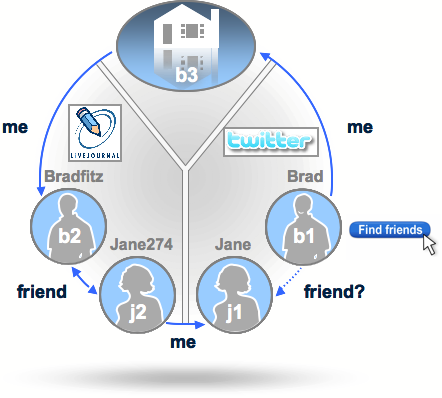
\includegraphics[scale=0.38]{../images/logos/find-a-friend.png}
        \column{.5\textwidth}
       Perhaps the most powerful aspect of \texttt{NetworkX} is its ability to work in Python to generate networks from live-streaming data
        \begin{itemize}
            \uncover<2->{\item In Python, use \texttt{NetworkX}, \texttt{cjson} and a other standard scientific libraries to parse Google's SocialGraph data }
            \uncover<3->{\item Using a ``seed'' user, we will build out a network}
            \uncover<4->{\item Through a process called ``k-snowball searching'' $seed\rightarrow friend\rightarrow\dots\rightarrow friend_{k}$}
            \uncover<5->{\begin{itemize}
                \scriptsize{\item Seed: \href{http://imichaeldotorg.livejournal.com/}{imichaeldotorg.livejournal.com}
                \item $k = 3$}
            \end{itemize}}
            \uncover<6->{\item \alert{Note the low value of $k$}}
        \end{itemize}
    \end{columns}
\end{frame}

\begin{frame}[fragile]
    \frametitle{The code, part 1}
    \begin{columns}
        \column{.5\textwidth}
        \begin{block}{\scriptsize{Loading the libraries and scraping egonet}}
            \begin{code}
\tiny{\alert<2>{from cjson import *
from urllib import *
from time import *
from scipy import array,unique
...}
if __name__ == "__main__":
    \alert<3>{seed="imichaeldotorg" 
    seed_url="http://"+seed+".livejournal.com"
    # 3.1 Scrape, parse and build seed's ego net
    sg=get_sg(seed_url)
    net,newnodes=create_egonet(sg)
    nx.write_pajek(net,"../../data/"+seed+"_ego.net")
    nx.info(net)}
                \end{code}
            \end{block}}
        \column{.5\textwidth}
\begin{code}
\uncover<7->{\tiny{Name:                  [`http://imichaeldotorg.livejournal.com/']
Type:                  DiGraph
Number of nodes:       5
Number of edges:       5
Average in degree:     1.0
Average out degree:    1.0}}
\end{code}
    \end{columns}
    \begin{block}{}
        \begin{code}
    \tiny{def get_sg(seed_url):
        \alert<4>{sgapi_url="http://socialgraph.apis.google.com/lookup?q="+seed_url+"&edo=1&edi=1&fme=1&pretty=0"}
        \alert<5>{try:}
            \alert<6>{furl=urlopen(sgapi_url)
            fr=furl.read()
            furl.close()
            return fr}
        \alert<5>{except IOError:
            print "Could not connect to website"
            print sgapi_url
            return {}}}
        \end{code}
    \end{block}    
\end{frame}

\begin{frame}[fragile]
    \frametitle{Build egonet and snowball}
    \begin{columns}
        \column{0.4\textwidth}
        \begin{block}{\scriptsize{Creating the egonet}}
            \begin{code}
\tiny{def create_egonet(s):
    \alert<2>{try:}
        \alert<3>{raw=decode(s)
        G=nx.DiGraph()
        pendants=[]
        n=raw['nodes']
        nk=n.keys()
        G.name=str(nk)
        pendants=[]}
        \alert<4>{for a in range(0,len(nk)):
            for b in range(0,len(nk)):
                if a!=b:
                    G.add_edge(nk[a],nk[b])}
        for k in nk:
            ego=n[k]
            \alert<5>{ego_out=ego['nodes_referenced']
            for o in ego_out:
                G.add_edge(k,o)
                pendants.append(o)}
            \alert<6>{ego_in=ego['nodes_referenced_by']
            for i in ego_in:
                G.add_edge(i,k)
                pendants.append(i)}
        \alert<7>{pendants=array(pendants,dtype=str)
        pendants.flatten()
        pendants=unique(pendants)
        return G,pendants}
    \alert<2>{except DecodeError:
    ...
    except KeyError:}}
            \end{code}
        \end{block}
        \column{0.6\textwidth}
        \begin{block}{\scriptsize{Rolling the snowball}}
            \begin{code}
\tiny{def snowball_round(G,seeds,myspace=False):
    \alert<8>{t0=time()}
    \alert<9>{if myspace:
        seeds=get_myspace_url(seeds)}
    sb_data=[]
    \alert<10>{for s in range(0,len(seeds)):
        s_sg=get_sg(seeds[s])
        new_ego,pen=create_egonet(s_sg)
        for p in pen:
                sb_data.append(p)}
        \alert<11>{if s<1:
            sb_net=nx.compose(G,new_ego)
        else:
            sb_net=nx.compose(new_ego,sb_net)
        del new_ego}
        \alert<8>{if s==round(len(seeds)*0.2):
            sb_net.name='20% complete'
            nx.info(sb_net)
            print 'AT: '+strftime('%m/%d/%Y, %H:%M:%S', gmtime())
            print ''
    ...
    # More time keeping, probably a MUCH better way to do this}
    \alert<12>{sb_data=array(sb_data)
    sb_data.flatten()
    sb_data=unique(sb_data)
    nx.info(sb_net)
    return sb_net,sb_data}}
            \end{code}
        \end{block}
    \vspace{5mm}
    \end{columns}
\end{frame}

\begin{frame}[fragile]
    \frametitle{Build the whole network}
    \begin{columns}
        \column{0.5\textwidth}
         \scriptsize{\begin{tabular}{l|l|l|l|l}
         Step & Nodes & Edges & Mean Degree & Density \\ \hline \hline
         \color<2>{red}{Seed} & \color<2>{red}{5} & \color<2>{red}{5} & \color<2>{red}{2.0} & \color<2>{red}{0.25} \\ \hline
         \color<3>{red}{$k=2$} & \color<3>{red}{75} & \color<3>{red}{115} & \color<3>{red}{3.0} & \color<3>{red}{0.02} \\ \hline
         \color<4>{red}{$k=3$} & \color<4>{red}{4,938} & \color<4>{red}{8,659} & \color<4>{red}{3.5} & \color<4>{red}{$3.6(10^{-4})$}
         \end{tabular}}
         \column{0.5\textwidth}
         \begin{itemize}
            \item \uncover<2->{\scriptsize{Our seed is abnormally isolated, with only four neighbors}}
            \item \uncover<3->{\scriptsize{Large jump after first snowball}}
            \item \uncover<4->{\scriptsize{Massive structural leap at $k=3$}}
         \end{itemize}
    \end{columns}
    \begin{center}
        \uncover<3->{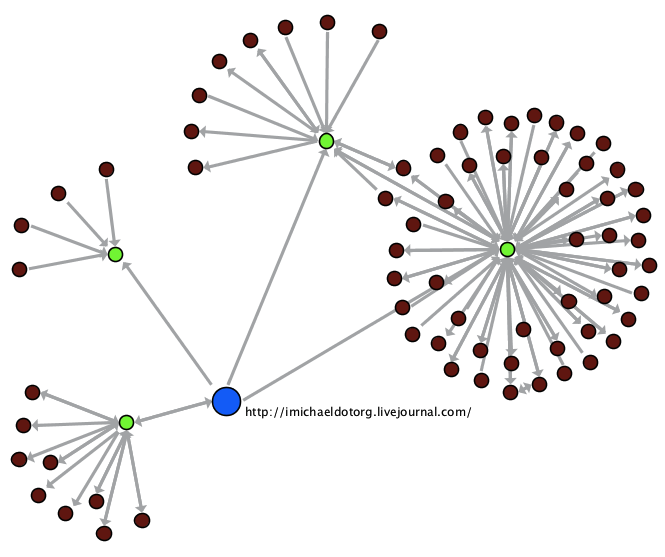
\includegraphics[scale=0.3]{../images/networks/goog_api_k2.png}}
    \end{center}
\end{frame}

\begin{frame}[fragile]
    \frametitle{The full network}
    To get a feeling for the size of the full network...
    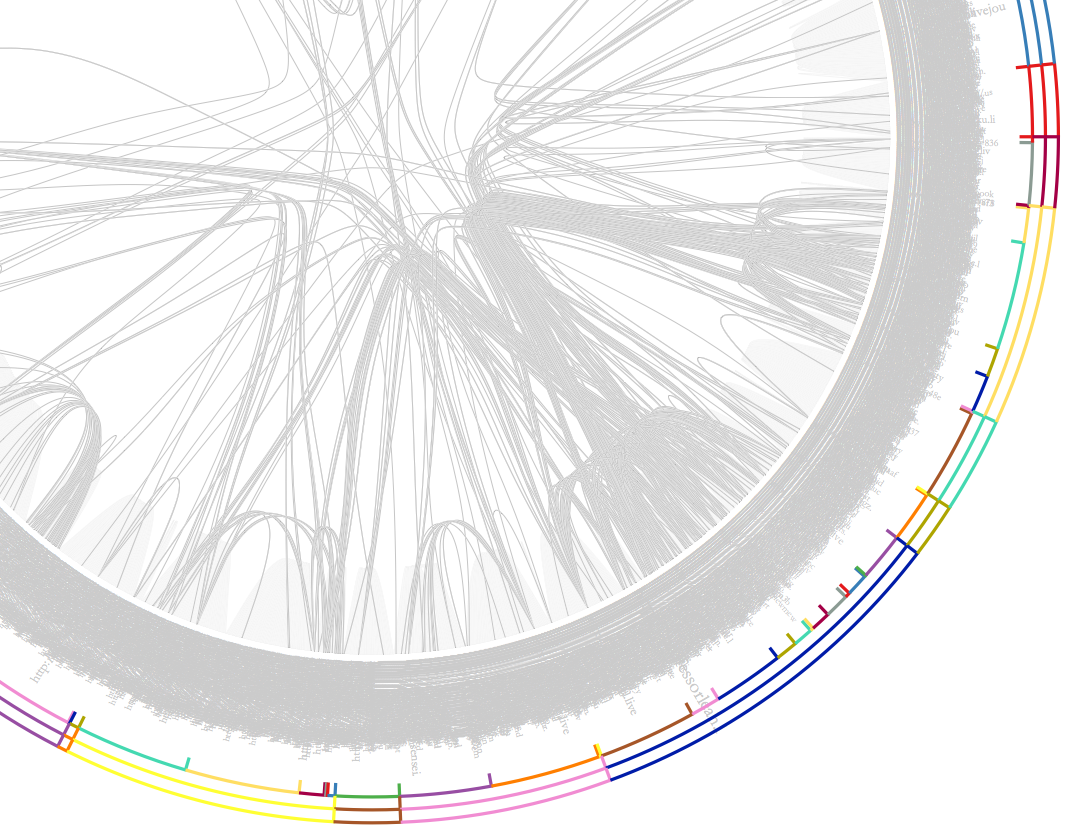
\includegraphics[scale=0.3]{../images/networks/big_wheel.png}
\end{frame}

% subsection building_directly_from_the_internet (end)

% section loading_data_from_multiple_sources (end)

\section{The Python \texttt{dict}} % (fold)
\label{sec:the_python_dict}

\subsection{Overview of the \texttt{dict} data type} % (fold)
\label{sub:overview_of_the_dict}

\begin{frame}[fragile]
    \frametitle{Python Dictionaries}
    \uncover<1->{The \texttt{dict} type is a data structure that represents a key$\rightarrow$value mapping}
    \uncover<2->{\begin{block}{Working with the dict type}}
        \begin{code}
\uncover<2->{\alert<2>{\# Keys and values can be of any data type}}
\uncover<2->{>>> fruit\_dict=\{"apple":1,"orange":[0.23,0.11],"banana":True \}} \newline
\uncover<3->{\alert<3>{\# Can retrieve the keys and values as Python lists (vector)}
>>> fruit\_dict.keys()
["orange","apple","banana"]} \newline
\uncover<4->{\alert<4>{\# Or create a (key,value) tuple}
>>> fruit\_dict.items()
[("orange",[0.23,0.11]),("apple",1),("Banana",True)]}
\uncover<5->{\alert<5>{\# This becomes especially useful when you master Python ``list comprehension''}}
            \end{code}
        \end{block}
\uncover<6->{The Python dictionary is an extremely flexible and useful data structure, making it one of the primary advantages of Python over other languages
\begin{itemize}
    \item This is particularly useful when performing analysis on networks, where node labels are natural keys
\end{itemize}}
\uncover<7->{\begin{center}
    \alert{Now, try creating a \texttt{dict} of your own}
\end{center}}
\end{frame}

% subsection overview_of_the_dict (end)

\subsection{How NetowrkX uses the \texttt{dict}} % (fold)
\label{sub:how_netowrkx_uses_the_dict}

\begin{frame}[fragile]
    \frametitle{Using dictionaries for network analysis}
    \begin{columns}
        \column{.45\textwidth}
        From the documentation...\\ \vspace{3mm}
        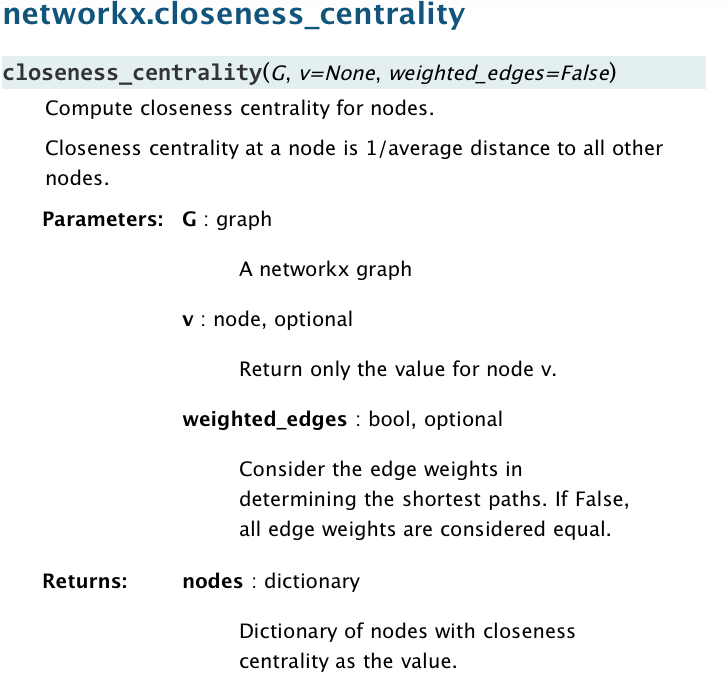
\includegraphics[width=5cm]{../images/figures/closeness_doc.png}
        \column{.55\textwidth}
        \texttt{NetworkX}'s metric's make extensive use of the dict type
        \begin{itemize}
            \item In this case the key$\rightarrow$value mapping is of the form: \texttt{\{node\_label: metric\}} 
        \end{itemize}
        Let's look at an example:
        \begin{block}{}
            \begin{code}
\scriptsize{>>> in_cen=nx.in_degree_centrality(hartford)
>>> in_cen
\{1: 0.014218009478672987, 2: 0.018957345971563982,...
...
90: 0.0047393364928909956, 293: 0.0\}}
            \end{code}
        \end{block}
        We can see that node \#90 has in-degree centrality 0.0047
        \begin{itemize}
            \item But we can do so much more!
        \end{itemize}
    \end{columns}
\end{frame}

% subsection how_netowrkx_uses_the_dict (end)

% section the_python_dict (end)

\section{Running basic centralities} % (fold)
\label{sec:running_basic_centralities}

\subsection{Calculating centralities} % (fold)
\label{sub:calculating_centralities}

\begin{frame}[fragile]
    \frametitle{Running multiple measures}
    For our first analysis in \texttt{NetworkX}, we will do some basic network manipulation, then run multiple measures to find highest centrality nodes
    \begin{itemize}
        \item First, we will need to convert to an undirected network, and extract the main component
    \end{itemize}
    \begin{block}{}
        \begin{code}
# Many of the centrality metrics require undirected graphs, so we will symmetrize
>>> \alert<2>{hartford_ud=hartford.to_undirected()}
# The network also has many small components, but for
# this analysis we are interested in the largest
>>> \alert<3>{hartford_mc=hartford_main=nx.connected_component_subgraphs(hartford_ud)[0]}
        \end{code}
    \end{block}
    Next, we will calculate multiple measures
    \begin{block}{}
        \begin{code}
# Betweenness centrality
>>> \alert<4>{bet_cen=nx.betweenness_centrality(hartford_mc)}
# Closeness centrality
>>> \alert<4>{clo_cen=nx.closeness_centrality(hartford_mc)}
# Eigenvector centrality
>>> \alert<4>{eig_cen=nx.eigenvector_centrality(hartford_mc)}
        \end{code}
    \end{block}
\end{frame}

\begin{frame}[fragile]
    \frametitle{Finding most central actors}
    To find the most central actors we will use Python's list comprehension technique to do basic data manipulation on our centrality dictionaries
    \begin{columns}
        \column{.57\textwidth}
            \begin{block}{}
        \begin{code}
def highest_centrality(cent_dict):
    """Returns node key with largest value from
    NX centrality dict"""
    \alert<2>{# Create ordered tuple of centrality data
    cent_items=cent_dict.items()}
    \alert<3>{# List comprehension!
    cent_items=[(b,a) for (a,b) in cent_items]}
    \alert<4>{# Sort in descending order
    cent_items.sort()
    cent_items.reverse()
    return cent_items[0][1]}
        \end{code}
            \end{block}
            \column{.43\textwidth}
            \uncover<3->{List comprehension
            \begin{itemize}
                \scriptsize{\item Given a dict: \texttt{d=\{1: 0.15, 2: 0.67\}}}
                \scriptsize{\item \texttt{d.items()} $\rightarrow$ \texttt{[(1,0.15),(2,0.67)]}}
                \scriptsize{\item \texttt{d=[(b,a) for (a,b in d)]} $\rightarrow$ \texttt{[(0.15,1),(0.67,2)]}}
            \end{itemize}}}
            \uncover<4->{Here, we use list comprehension in order to use Python's built-in \texttt{sort} and \texttt{reverse} list functions}
    \end{columns}
    \vspace{2mm}Now, just ask for the answer
    \begin{block}{Finding Most central actors}
        \begin{code}
\scriptsize{>>>  print("Actor "+str(highest_centrality(bet_cen))+" has the highest Betweenness centrality")
\alert<5->{Actor 82 has the highest Betweenness centrality}}
        \end{code}
    \end{block}
\end{frame}

\begin{frame}[fragile]
    \frametitle{Calculating degree distribution}
    One of the most popular network level statistical description of a network is its degree distribution
    \begin{itemize}
        \item In \texttt{NetworkX} this is a simply one-line operation
    \end{itemize}
    \begin{columns}
        \column{.6\textwidth}
         \begin{block}{Get list of degree rank frequency}
                \begin{code}
# Create a Barabasi-Albert network
>>> ba_net=barabasi_albert_graph(1000,2)   
# 6.1 Built-in function for degree distribution
>>> dh=degree_histogram(ba_net)
                \end{code}
         \end{block}
         \uncover<2->{\begin{itemize}
            \item As we will see next, we can use \texttt{matplotlib} to take this data and create publication ready plots
            \item Ex. from \url{http://networkx.lanl.gov/examples/drawing/degree_histogram.html}
         \end{itemize}}
         \column{.4\textwidth}
            \uncover<2->{\includegraphics[width=5cm]{../images/figures/BA_1000.png}}
    \end{columns}
\end{frame}


% subsection calculating_centralities (end)

\subsection{Calculating basic community structure} % (fold)
\label{sub:calculating_basic_community_structure}

\begin{frame}[fragile]
    \frametitle{Calculating basic community structure}
    Often in network analysis we are interested in estimating the cohesiveness of a network, or the communities that exists within the structure
    \vspace{3mm}
    
    \uncover<2->{\textbf{Cliques}
    \begin{itemize}
        \item Maximal cliques are the largest complete subgraph containing a given point.  There are several algorithms for finding cliques, including Bron & Kerbosch (1973), Tomita, Tanaka and Takahashi (2006), Cazals and Karande (2008)
    \end{itemize}}
    \uncover<3->{\textbf{Clustering}
    \begin{itemize}
        \item For each node find the fraction of possible triangles that exist,$c_{v}=\frac{2T(v)}{deg(v)(deg(v)-1)}$, where $T(v)$ is the number of triangles through node $v$.
    \end{itemize}}
    \uncover<4->{\textbf{Transitivity}
    \begin{itemize}
        \item The fraction of all possible triangles which are in fact triangles. Or, $Trans=3\left(\frac{T}{t}\right)$, where $T=$ \# of possible triangles and $t=$ \# of actual triads
    \end{itemize}}
    \uncover<5->{We will use clustering coefficients to identify community structure in the Hartford drug network}
\end{frame}

\begin{frame}[fragile]
    \frametitle{Toy community detection example (not a good one)}
    \begin{block}{Calculating clustering coefficients}
        \begin{code}
\scriptsize{\alert<2>{# Calculate clustering coefficients of each node (return as dict)
clus=clustering(hartford_mc,with_labels=True)}
\alert<3>{# Get counts of nodes membership for each clustering coefficient, and clean up
unique_clus=list(unique(clus.values()))
clus_counts=zip(map(lambda c: clus.values().count(c),unique_clus),unique_clus)
clus_counts.sort()
clus_counts.reverse()}
\alert<4>{# Create a subgraph from nodes with most frequent clustering coefficient
mode_clus_sg=subgraph(hartford_mc,[(a) for (a,b) in clus.items() if b==clus_counts[0][1]])}}         
        \end{code}
    \end{block}
    \begin{columns}
        \column{.5\textwidth}
        \begin{itemize}
            \uncover<2->{\item Use the \texttt{with\_labels} to return a \texttt{dict} keyed by node label}
            \uncover<3->{\item The \texttt{zip} function takes two \texttt{lists} and returns a \texttt{tuple}}
            \uncover<4->{\item More complex list comprehension with logic operator}
        \end{itemize}
        \column{.5\textwidth}
            \begin{center}
                \uncover<5->{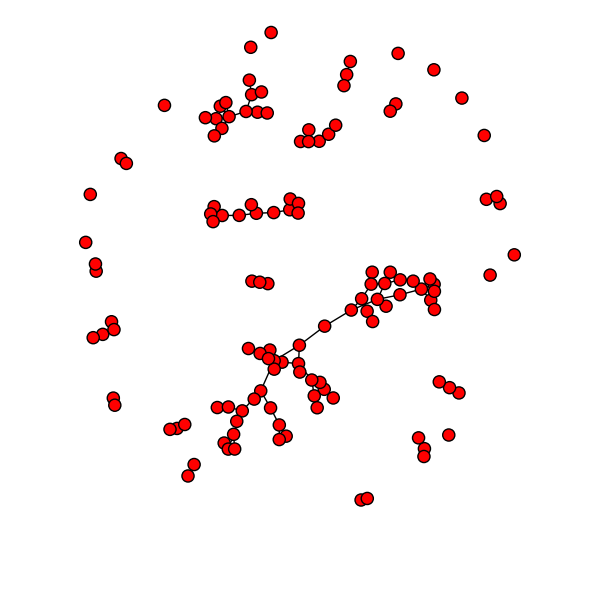
\includegraphics[width=3cm,clip,trim=2cm 2cm 2cm 2cm]{../images/networks/mode_clus_sg.png}}
            \end{center}
    \end{columns}
    \begin{center}
        \uncover<6->{\alert{Later, we'll learn how to create a network visualization like the one above}}
    \end{center}
\end{frame}


% subsection calculating_basic_community_structure (end)

\subsection{Visualizing analysis with \texttt{matplotlib}} % (fold)
\label{sub:visualizing_analysis_with_matplotlib}

\begin{frame}[fragile]
    \frametitle{Introduction to \texttt{matplotlib}}
    Recall Python's scientific computing trinity: \texttt{NumPy}, \texttt{SciPy} and \texttt{matplotlib}
    \begin{itemize}
        \item While \texttt{NumPy} and \texttt{SciPy} do most of the behind the scenes work, you will interact with \texttt{matplotlib} frequently for when doing network analysis
    \end{itemize}
    \begin{columns}
        \column{.55\textwidth}
            \uncover<2->{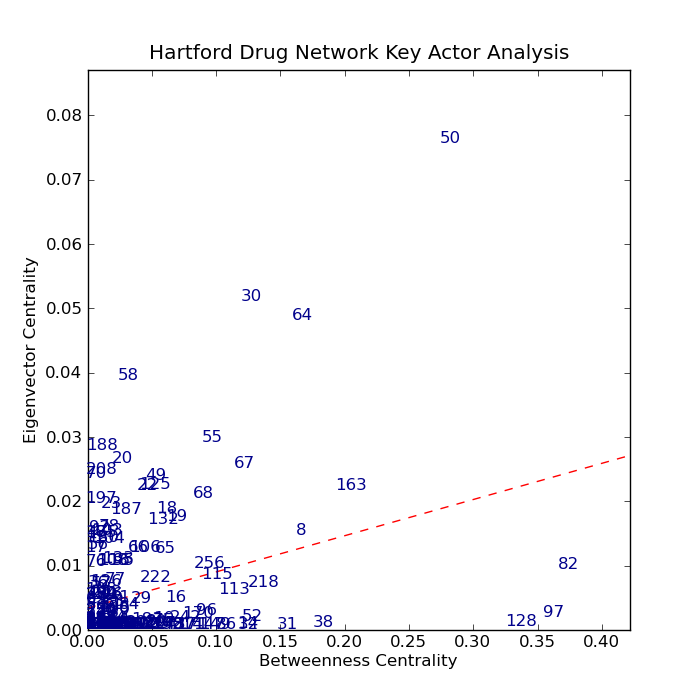
\includegraphics[width=6.2cm]{../images/figures/drug_scatter.png}}
        \column{.45\textwidth}
        \uncover<3->{We will need to create a function that takes two centrality \texttt{dict} and generates this plot}
        \begin{enumerate}
            \uncover<4->{\item Create a \texttt{matplotlib} figure}
            \uncover<5->{\item Plot each node label as a point}
            \uncover<6->{\item Add a ``best fit'' line}
            \uncover<7->{\item Add axis and title labels}
            \uncover<8->{\item Save figure as a PNG file}
        \end{enumerate}
    \end{columns}
\end{frame}

\begin{frame}[fragile]
    \frametitle{Creating a key actor plot in \texttt{matplotlib}}
        \begin{block}{The \texttt{centrality\_scatter} function, part one}
            \begin{code}
\scriptsize{def centrality_scatter(met_dict1,met_dict2,path="",ylab="",xlab="",title="",reg=False):
    \alert<2>{# Create figure and drawing axis
    fig=P.figure(figsize=(7,7))
    ax1=fig.add_subplot(111)}
    \alert<3>{# Create items so actors can be sorted properly
    met_items1=met_dict1.items()
    met_items2=met_dict2.items()
    met_items1.sort()
    met_items2.sort()
    # Grab data
    xdata=[(b) for (a,b) in met_items1]
    ydata=[(b) for (a,b) in met_items2]}
    \alert<4>{# Add each actor to the plot by ID
    for p in xrange(len(met_items1)):
        ax1.text(x=xdata[p],y=ydata[p],s=str(met_items1[p][0]),color="indigo")}}
            \end{code}
        \end{block}
    \begin{itemize}
        \uncover<2->{\item Create a canvas to draw on}
        \uncover<3->{\item manipulate and store centrality data}
        \uncover<4->{\item Add points to plot as node labels}
    \end{itemize}
\end{frame}

\begin{frame}[fragile]
    \frametitle{Creating a key actor plot in \texttt{matplotlib}}
    \begin{block}{The \texttt{centrality\_scatter} function, part one}
        \begin{code}
\scriptsize{def centrality_scatter(met_dict1,met_dict2,path="",ylab="",xlab="",title="",reg=False):
...
    \alert<2>{# If adding a best fit line, we will use NumPy to calculate the points.
    if reg:
        # Function returns y-intercept and slope.  So, we create a function to 
        # draw LOBF from this data
        slope,yint=polyfit(xdata,ydata,1)
        xline=P.xticks()[0]
        yline=map(lambda x: slope*x+yint,xline)
        # Add line
        ax1.plot(xline,yline,ls='--',color='grey')}
    \alert<3>{# Set new x- and y-axis limits to data
    P.xlim((0.0,max(xdata)+(.15*max(xdata))))   # Give a little buffer
    P.ylim((0.0,max(ydata)+(.15*max(ydata))))}
    \alert<4>{# Add labels
    ax1.set_title(title)
    ax1.set_xlabel(xlab)
    ax1.set_ylabel(ylab)
    # Save figure
    P.savefig(path,dpi=100)}}
        \end{code}
    \end{block}
    \scriptsize{\begin{itemize}
        \uncover<2->{\item Add a best fit line}
        \uncover<3->{\item Resize figure to fit data}
        \uncover<4->{\item Add labels, and save the figure as a PNG file}
    \end{itemize}}
\end{frame}


% subsection visualizing_analysis_with_matplotlib (end)

% section running_basic_centralities (end)

\section{Getting things out of \texttt{NetworkX}} % (fold)
\label{sec:getting_things_out_of_networkx}

\subsection{Outputting network data} % (fold)
\label{sub:outputting_network_data}

\begin{frame}[fragile]
    \frametitle{Exporting network data and analytics}
    As powerful as \texttt{NetworkX} and the complementing scientific computing packages in Python are, it may often be useful or necessary to output your data for additional analysis
    \begin{itemize}
        \uncover<2->{\item Suite of tools lacks your specific need}
        \uncover<3->{\item Require alternate visualization}
        \uncover<4->{\item Storage for later analysis}
    \end{itemize}
    \uncover<5->{In most cases this will entail either exporting the raw network data, or metrics from some network analysis}
    \begin{enumerate}
        \uncover<6->{\item \texttt{NetworkX} can write out network data in as many formats as it can read them, and the process is equally straightforward}
        \uncover<7->{\item When you want to export metrics we can use Python's built-in \texttt{XML} and \texttt{CSV} libraries}
        \uncover<8->{\item Depending on your needs you may prefer one, the other or both}
    \end{enumerate}
    \uncover<9->{Next, we will review how to save data in different formats and export metrics to a \texttt{CSV} file using the Hartford drug net data}
\end{frame}

\begin{frame}[fragile]
    \frametitle{Saving network data in different formats}
    The syntax for exporting network data follows exactly the syntax for loading it
    \begin{block}{NX syntax for writing a network file}
        \begin{tabular}{cccc}
        $>>>$ & \alert<2>{nx.write\_format(G}, & \alert<3>{``path/to/file.txt''}, & \alert<4>{\emph{...options...}}) \\
        & \alert<2>{\uparrow} & \alert<3>{\uparrow} & \alert<4>{\uparrow} \\
        & \alert<2>{\scriptsize{NX function, net variable}} & \alert<3>{\scriptsize{File to be written}} & \alert<4>{\scriptsize{Nodes/edge data, etc.}}
        \end{tabular}
    \end{block}
    \uncover<5->{Let's try!
    \begin{itemize}
        \item Output the Hartford drug net data as an adjacency list
        \item Add metric data to each node of the network 
        \item Output new network in Pajek format with node attributes
    \end{itemize}}
\end{frame}

\begin{frame}[fragile]
    \frametitle{Saving network data and adding node attributes}
    As shown, this is a simple one line operation
    \begin{block}{Output Hartford drug net data as an adjacency list}
        \begin{code}
nx.write_adjlist(hartford_mc,"../../data/hartford_mc_adj.txt")
        \end{code}
    \end{block}
    Next, we will add the Eigenvector centrality of each node to the graph object
    \begin{block}{Adding node attributes}
        \begin{code}
def add_metric(G,met_dict):
    """Adds metric data to G from a dictionary keyed by node labels"""
    \alert<2>{if(G.nodes().sort()==met_dict.keys().sort()):}
        \alert<3>{for i in met_dict.keys():
            G.add_node(i,metric=met_dict[i])
        return G}
    \alert<2>{else:
        raise ValueError("Node labels do not match")}
        \end{code}
    \end{block}
    \begin{itemize}
        \uncover<2->{\item Quick error checking}
        \uncover<3->{\item Add node attribute as ``metric''}
    \end{itemize}
\end{frame}


% subsection outputting_network_data (end)

\subsection{Exporting metric data} % (fold)
\label{sub:exporting_metric_data}

\begin{frame}[fragile]
    \frametitle{Using the Python \texttt{CSV} library}
    Python has powerful built-in tools for reading and writing standard data formats
    \begin{itemize}
        \item One of the most useful, and frequently used, is the \texttt{CSV} library and the \texttt{DictWriter}
    \end{itemize}
    \begin{block}{}
        \begin{code}
\scriptsize{\alert<2>{import csv}
...
def csv_exporter(\alert<3>{data_dict,path}):
    """Takes a dict of centralities keyed by column headers and exports 
    data as a CSV file"""
    \alert<4>{# Create column header list
    col_headers=["Actor"]
    col_headers.extend(data_dict.keys())}
    \alert<5>{# Create CSV writer and write column headers
    writer=csv.DictWriter(open(path,"w"),fieldnames=col_headers)
    writer.writerow(dict((h,h) for h in col_headers))}
    \alert<6>{# Write each row of data
    for j in data_dict[col_headers[1]].keys():}
        \alert<7>{# Create a new dict for each row
        row=dict.fromkeys(col_headers)
        row["Actor"]=j
        for k in data_dict.keys():
            row[k]=data_dict[k][j]
        writer.writerow(row)}}
        \end{code}
    \end{block}
\end{frame}

\begin{frame}[fragile]
    \frametitle{The results of CSV export}
    \begin{columns}
        \column{.5\textwidth}
        We can now open the \texttt{CSV} file in our favorite spreadsheet program
        \begin{itemize}
            \item Perform traditional data exploration
            \item Load into other analytics platforms for additional analysis (e.g., \texttt{R})
            \item Store for latter use
        \end{itemize}
        \column{.5\textwidth}
        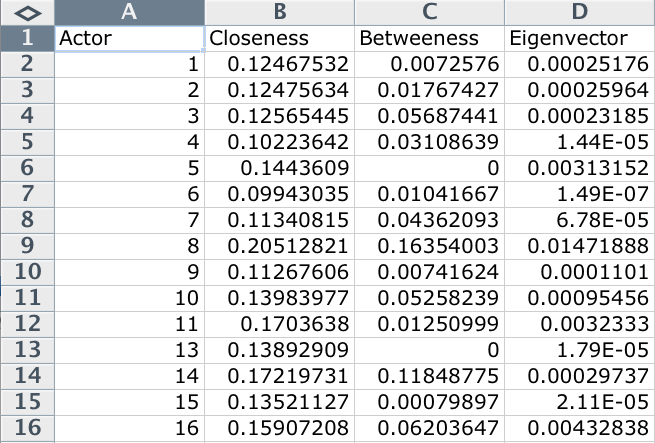
\includegraphics[width=5.5cm]{../images/figures/metrics_screen_shot.png}
    \end{columns}
\end{frame}

% subsection exporting_metric_data_as_csv (end)

% section getting_things_out_of_networkx (end)

\section{Basic visualization} % (fold)
\label{sec:basic_visualization}

\subsection{Network visualization algorithms} % (fold)
\label{sub:network_visualization_algorithms}

\begin{frame}[fragile]
    \frametitle{What makes a good network visualization technique}
    Development of visualization techniques and algorithms has become somewhat of a cottage industry
    \uncover<2->{\begin{itemize}
        \item Maximize ``visibility'' of network
        \item Scale up to very large graphs
        \item Display nodal- (centrality) of network-level (community structure) information
    \end{itemize}}
    \uncover<3->{\texttt{NetworkX} was designed as a data manipulation and analysis tool, and therefore is not meant as a visualization platform}
    \uncover<4->{\begin{itemize}
        \item \alert{It is, however, still capable of making very nice visualization}
    \end{itemize}
    \begin{tabular}{ccc}
        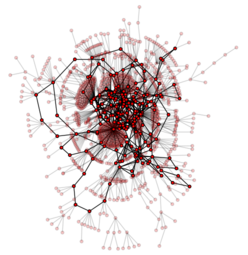
\includegraphics[width=3cm]{../images/networks/art1.png} & 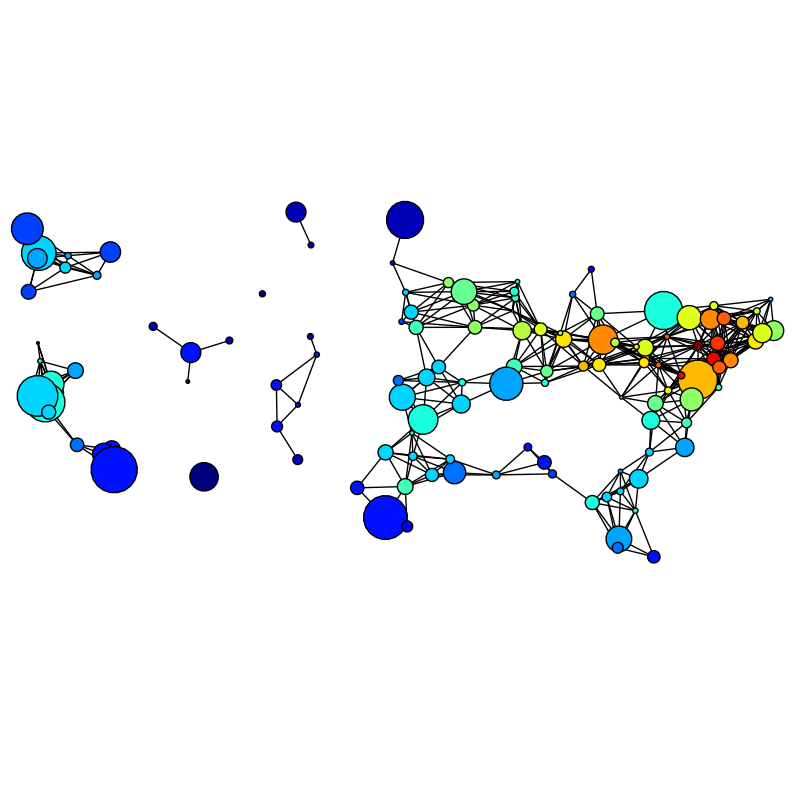
\includegraphics[width=3cm]{../images/networks/knuth_miles.png} & 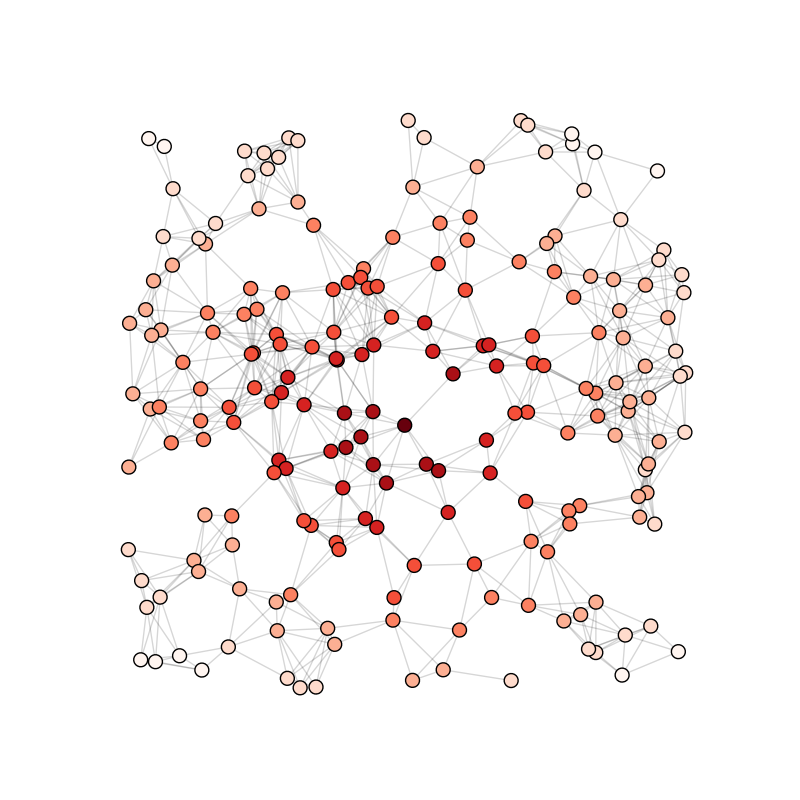
\includegraphics[width=3cm]{../images/networks/random_geometric_graph.png}
    \end{tabular}}
\end{frame}

\begin{frame}[fragile]
    \frametitle{Visualization algorithms in \texttt{NetworkX} - Random \& Circle}
    The most basic visualization techniques are the random and circular layouts
    \begin{itemize}
        \item The random layout places nodes in...random positions
        \item The circular layout places nodes in...a circle
    \end{itemize}
    \begin{center}
        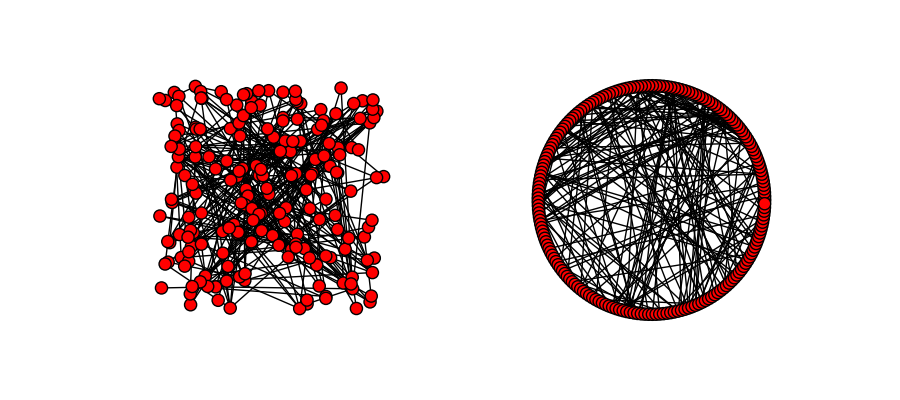
\includegraphics[width=6cm,clip,trim=2cm 2cm 2cm 2cm]{../images/networks/rand_circ.png}
    \end{center}
    \begin{block}{}
        \begin{code}
# Use subplots to draw random and circular layouts
# of drug net side-by-side
\alert<2>{fig1=P.figure(figsize=(9,4))
fig1.add_subplot(121)}
\alert<3>{nx.draw_random(hartford_mc,with_labels=False,node_size=60)}
\alert<4>{fig1.add_subplot(122)
nx.draw_circular(hartford_mc,with_labels=False,node_size=60)
P.savefig("../../images/networks/rand_circ.png")}
        \end{code}
    \end{block}
\end{frame}

\begin{frame}[fragile]
    \frametitle{Visualization algorithms in \texttt{NetworkX} - Spring \& Spectral}
    \begin{columns}
        \column{.5\textwidth}
        More commonly used visualization techniques include the spring and spectral layouts
        \begin{itemize}
            \uncover<2->{\item The spring layout is a version of the Fruchterman-Reingold force-directed algorithm, which attempts to minimize overlapping edges}
            \uncover<3->{\item The spectral layout finds node position using the eigenvectors of the graph Laplacian, which is useful for quickly visualizing structural clustering}
        \end{itemize}
        \column{.5\textwidth}
        \begin{center}
            \uncover<2->{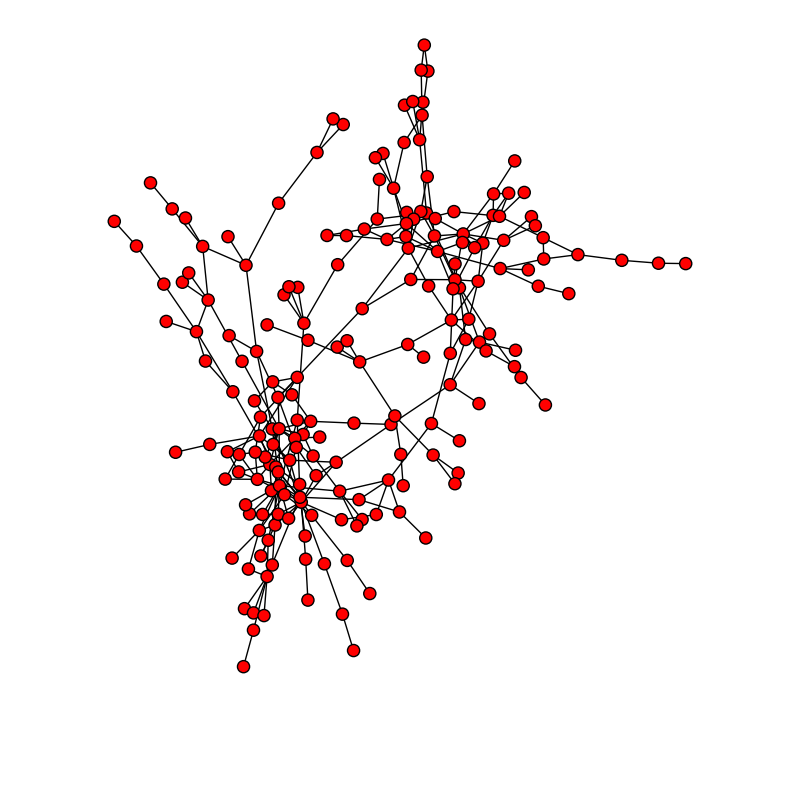
\includegraphics[width=3.5cm,clip,trim=2cm 2cm 2cm 2cm]{../images/networks/spring.png} \\}
            \uncover<3->{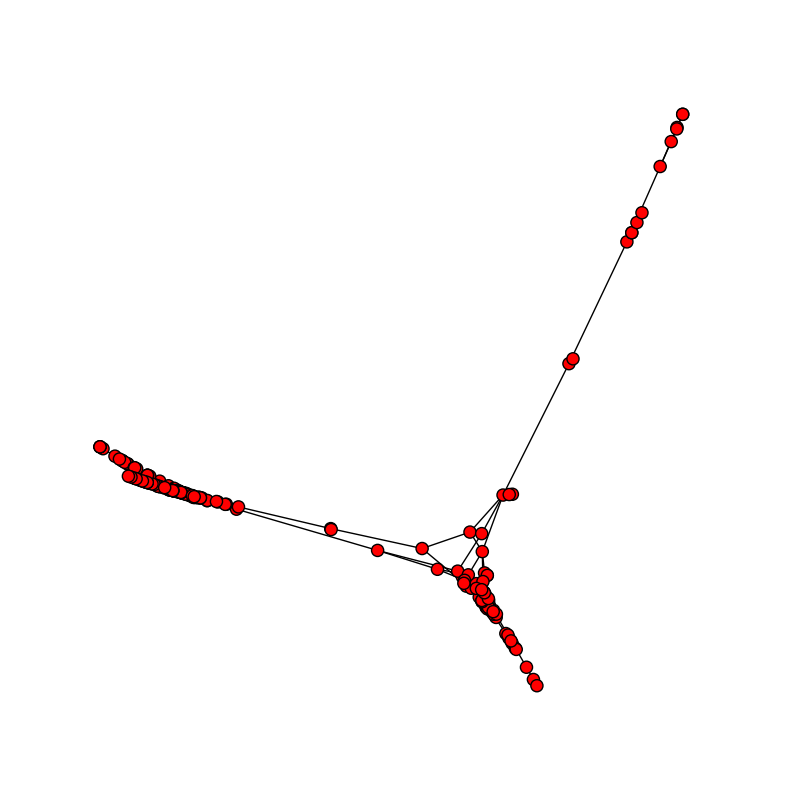
\includegraphics[width=3.5cm,clip,trim=2cm 2cm 2cm 2cm]{../images/networks/spectral.png}}
        \end{center}
    \end{columns}
\end{frame}

\begin{frame}[fragile]
    \frametitle{Visualization algorithms in \texttt{NetworkX} - Shell}
    The shell layout draws nodes as concentric circles
    \begin{itemize}
        \item Two dimensional extension of the circle layout
        \item We may have some reason to isolate certain nodes
    \end{itemize}
    \begin{columns}
        \column{.7\textwidth}
            \begin{block}{25th percentile Eigenvector centrality actors}
                \begin{code}
\scriptsize{P.figure(figsize=(8,8))
\alert<2>{# Find actors in 25th percentile
max_eig=max([(b) for (a,b) in eig_cen.items()])
s1=[(a) for (a,b) in eig_cen.items() if b>=.25*max_eig]
s2=hartford_mc.nodes()}
\alert<3>{# setdiff1d is a very useful NumPy function!
s2=list(setdiff1d(s2,s1))       
shells=[s1,s2]}    
\alert<4>{# Calculate position and draw          
shell_pos=shell_layout(hartford_mc,shells)
draw_networkx(hartford_mc,shell_pos,with_labels=False,node_size=60)
P.savefig("../../images/networks/shell.png")}}
                \end{code}
            \end{block}
        \column{.3\textwidth}
            \uncover<5->{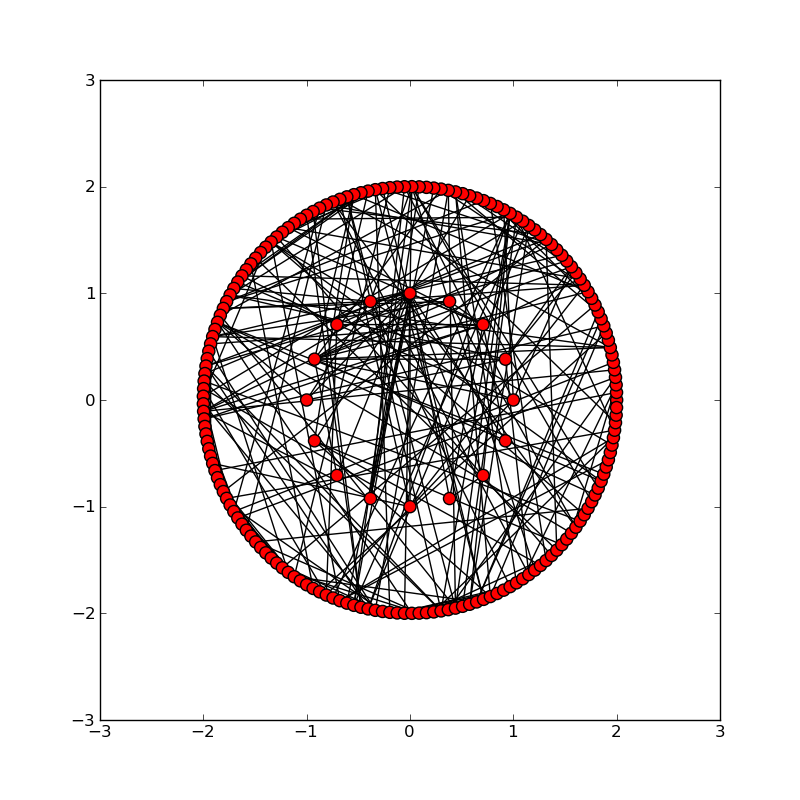
\includegraphics[width=3.8cm,clip,trim=4cm 4cm 4cm 4cm]{../images/networks/shell.png}}
    \end{columns}
    \vspace{2mm}
    \uncover<6->{Beyond layout, we may also want to add analytical data to our visualization}
\end{frame}

% subsection network_visualization_algorithms (end)

\subsection{Adding analysis to visualization} % (fold)
\label{sub:adding_analysis_to_visualization}

\begin{frame}[fragile]
    \frametitle{Changing node and edge size and colors}
    \texttt{NetworkX} allows you to alter the size, color and shape of the nodes and edges in any visualization
    \uncover<2->{\begin{itemize}
        \item This can be particularly useful if we want to make some actors more prominent than others
    \end{itemize}}
    \uncover<3->{In our final exercise, we will add the following analysis to the Hartford drug network
    \begin{itemize}
        \item Node size by Eigenvector centrality
        \item Intensity of node color by betweenness centrality
        \item Edge thickness by edge betweenness
    \end{itemize}}
\end{frame}

\begin{frame}[fragile]
    \frametitle{The code to add analysis to visualization}
    \begin{block}{More list comprehension and \texttt{matplotlib} colormaps}
        \begin{code}
\alert<2>{# Adding analysis to visualization
P.figure(figsize=(15,15))
P.subplot(111,axisbg="lightgrey")
spring_pos=nx.spring_layout(hartford_mc,iterations=1000)}
\alert<3>{# Use betweeneess centrality for node color intensity
bet_color=bet_cen.items()
bet_color.sort()
bet_color=[(b) for (a,b) in bet_color]}
\alert<4>{# Use Eigenvector centrality to set node size
eig_size=eig_cen.items()
eig_size.sort()
eig_size=[((b)*2000)+20 for (a,b) in eig_size]}
\alert<5>{# Use matplotlib's colormap for node intensity 
draw_networkx(hartford_mc,spring_pos,node_color=bet_color,...
    ...cmap=P.cm.Greens,node_size=eig_size,with_labels=False)
P.savefig("../../images/networks/analysis.png")}
        \end{code}
    \end{block}
\end{frame}


\begin{frame}[fragile]
    \frametitle{Final visualization}
    \begin{center}
        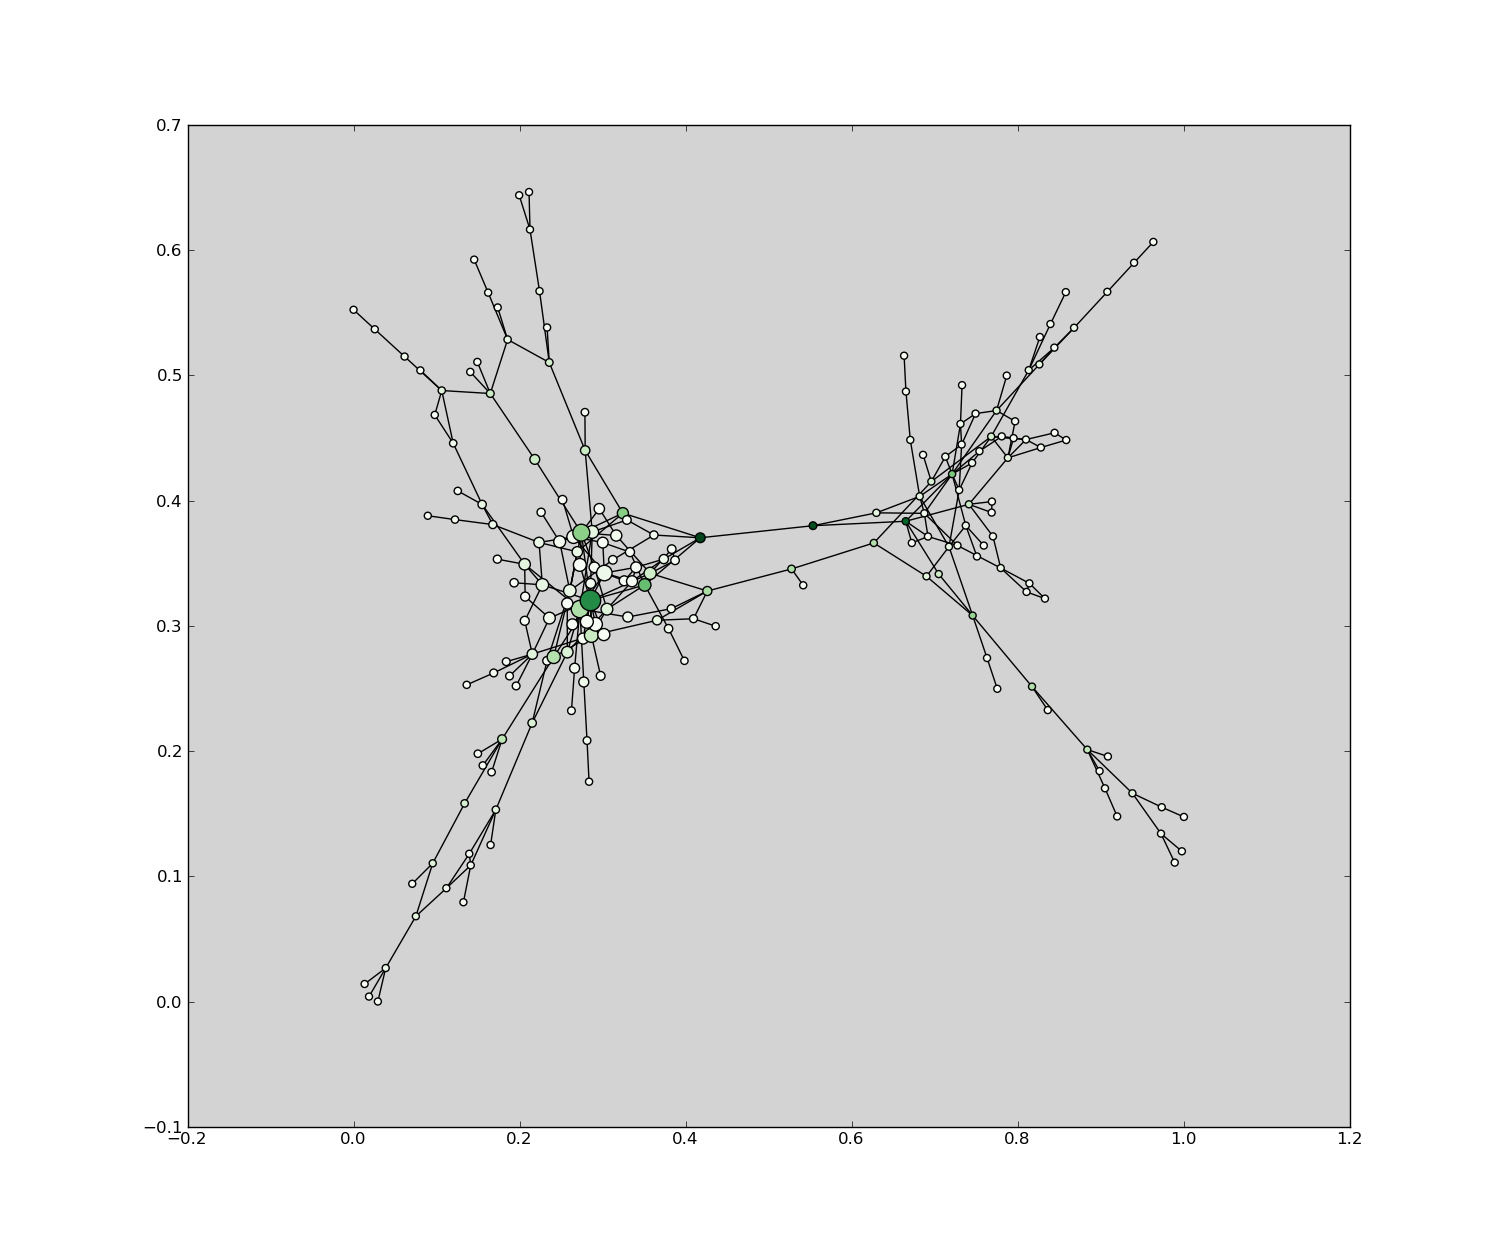
\includegraphics[width=9cm,clip,trim=5cm 5cm 4cm 4cm]{../images/networks/analysis.png}
    \end{center}
\end{frame}

% subsection adding_analysis_to_visualization (end)

% section basic_visualization (end)

\begin{frame}[plain]
    \frametitle{Module IV Review}
    Basic Analysis
    \begin{itemize}
        \uncover<2->{\item How to load local data, and an example of building networks from data streamed directly from the Internet}
        \uncover<3->{\item A brief review of the Python \texttt{dict} data type}
        \uncover<4->{\item Calculating basic metrics, how they are stored in \texttt{NetworkX} and how to manipulate them (list comps!)}
        \uncover<5->{\item How to use \texttt{matplotlib} to visualize our analysis}
        \uncover<6->{\item Getting data out of \texttt{NetworkX} both as raw network data or analytics using the \texttt{CSV} library}
        \uncover<7->{\item Network visualization techniques in \texttt{NetworkX} and how to add network analysis to a visualization}
    \end{itemize}
    \uncover<8->{\begin{center}
        \Huge{Questions?}
    \end{center}}
\end{frame}


\end{document}
